\begin{apendicesenv}

\partapendices

\chapter{Variáveis utilizadas na análise da ploidia embrionária}
\label{apendice:variaveis}

Este anexo descreve as variáveis utilizadas na planilha de dados referente ao desenvolvimento embrionário e sua relação com a ploidia. As variáveis incluem informações demográficas, temporais e morfológicas do embrião, bem como métricas de qualidade baseadas no sistema Gardner. Todos os tempos descritos abaixo são expressos em horas.

\begin{itemize}
  \item \textbf{Variáveis Gerais}
  \begin{itemize}
      \item \textbf{Id:} Identificador numérico de cada paciente.
      \item \textbf{Idade:} Idade da paciente no momento do procedimento.
      \item \textbf{Data da biópsia:} Data em que foi realizada a biópsia embrionária.
      \item \textbf{Embrião n.:} Identificação numérica do embrião dentro do ciclo de fertilização.
      \item \textbf{Estágio:} Dia de evolução no cultivo (5º dia ou 6º dia) \cite{ramalho2024}.
      \item \textbf{Morfo:} Classificação morfológica dos embriões baseada no estágio de expansão da blástula, estágio inicial do desenvolvimento embrionário que ocorre após a segmentação (divisões celulares iniciais) do zigoto. As notas de 1 a 5 são a expansão do embrião, com 1 sendo o menos expansivo e 5 o mais expansivo \cite{ramalho2024}.
      \item \textbf{KIDScore™:} Algoritmo combina variáveis morfocinéticas e parâmetros de desenvolvimento embrionário. A pontuação vai de 0 a 10 por conta de estarmos utilizando embriões de estado de blastocisto \cite{gazzo2020}. 
  \end{itemize}
\end{itemize}

\begin{itemize}
  \item \textbf{Variáveis Temporais}
  As variáveis temporais são baseadas nos intervalos de tempo entre eventos específicos durante o desenvolvimento do embrião:
  \begin{itemize}
    \item \textbf{st2:} Primeiro indício de movimentos citoplasmáticos antes da primeira citocinese. É a fase final da divisão celular, onde o citoplasma é dividido entre as duas células filhas \cite{ramalho2024}.
    \item \textbf{t2:} Tempo para 2 células. Tempo necessário para o embrião completar a primeira clivagem, ou seja, a divisão da célula-ovo (zigoto) em duas células, entre 24,3 – 27,9 horas após a fertilização \cite{cruz2012}.
    \item \textbf{t3:} Tempo para 3 células. Marca o momento em que o embrião se divide de duas para três células, entre 35,4 – 40,3 horas após a fertilização \cite{cruz2012}.
    \item \textbf{t4:} Tempo para 4 células. Transição do embrião para o estágio de quatro células.
    \item \textbf{t5:} Tempo para 5 células. Momento em que o embrião alcança o estágio de cinco células, entre 48,8 – 56,6 horas após a fertilização \cite{cruz2012}.
    \item \textbf{t8:} Tempo para 8 células.
    \item \textbf{tSC:} Tempo de formação do estágio de clivagem sincronizada (Time to Synchronized Compaction). Representa o tempo necessário para que o embrião, após atingir o estágio de 8 células, comece a apresentar compactação sincronizada. A compactação consiste na união mais forte das células embrionárias \cite{kato2021}.
    \item \textbf{tSB:} Tempo para o início da blastulação (Time to Start Blastulation). Tempo necessário para o embrião iniciar a formação do blastocisto \cite{kato2021}.
    \item \textbf{tB:} Tempo para o Blastocisto (Time to Blastocyst). Tempo que leva para o embrião alcançar o estágio de blastocisto completo, que é o último estágio de desenvolvimento embrionário antes da implantação no útero \cite{yuan2023}.
    \item \textbf{t2-st2:} Intervalo de tempo entre o T2 e o ST2. Esse intervalo é usado para avaliar a regularidade e a qualidade das divisões celulares no estágio inicial do desenvolvimento embrionário \cite{ramalho2024}.
    \item \textbf{cc2 (t3-t2):} Tempo necessário para que o embrião passe da divisão de 2 células (T2) para a divisão de 3 células (T3). É utilizado para avaliar a regularidade e a dinâmica do ciclo celular inicial do embrião \cite{ramalho2024}.
    \item \textbf{cc3 (t5-t3):} Tempo necessário para que o embrião passe da divisão de 3 células (T3) para a divisão de 5 células (T5). É utilizado como um indicador da dinâmica do ciclo celular \cite{ramalho2024}.
    \item \textbf{t5-t2:} Intervalo de tempo entre o estágio de 2 células (T2) e o estágio de 5 células (T5). É uma métrica importante para avaliar a eficiência das divisões celulares iniciais \cite{ramalho2024}.
    \item \textbf{s2 (t4-t3):} Intervalo de tempo necessário para que o embrião passe do estágio de 3 células (T3) para o estágio de 4 células (T4). Este parâmetro é usado para avaliar a regularidade da divisão celular \cite{ramalho2024}.
    \item \textbf{s3 (t8-t5):} Intervalo de tempo necessário para que o embrião passe do estágio de 5 células (T5) para o estágio de 8 células (T8). É usado para avaliar a sincronização e a regularidade do ciclo celular \cite{ramalho2024}.
    \item \textbf{tSC-t8:} Intervalo de tempo entre o estágio em que o embrião atinge a compactação inicial (tSC) e o estágio de 8 células (T8). É usado para avaliar a transição do embrião das divisões celulares iniciais para o início da compactação \cite{ramalho2024}.
    \item \textbf{tB-tSB:} Intervalo de tempo entre o estágio em que o embrião atinge o blastocisto inicial (tSB) e o estágio de blastocisto expandido (tB). Avalia o tempo necessário para que o embrião progrida do início da formação do blastocisto até a sua expansão completa \cite{ramalho2024}.
  \end{itemize}
\end{itemize}

\begin{itemize}
  \item \textbf{Variável de Resultado}
  \begin{itemize}
    \item \textbf{Ploidia:} Estado de ploidia do embrião, resultado final da análise.
  \end{itemize}
\end{itemize}


\chapter{Z-score normalization (standardization)}
\label{apendice:zscore}


O Z-Score é um indicador numérico que ilustra a conexão entre uma determinada quantia e a média de um conjunto de valores, expressa em termos de desvios padrão. Quando o Z-Score de um dado é zero, isso sugere que ela coincide com a média do conjunto. Um Z-Score de 1 indica que o valor está um desvio padrão acima da média, ao passo que valores negativos sugerem que estão abaixo da média. A normalização pelo Z-Score, também conhecida como padronização, pressupõe que os dados sigam uma distribuição gaussiana (em forma de sino) e transforma os valores para que tenham uma média (\(\mu\)) de 0 e um desvio padrão (\(\sigma\)) de 1, facilitando a análise e a comparação entre variáveis com diferentes escalas \cite{jaiswal2024, maiseretorno2022}. A fórmula para padronização é:

\begin{center}
  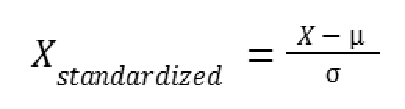
\includegraphics[scale=0.8]{figuras/Z-Score.pdf}
\end{center}


Em que:
\begin{itemize}
  \item \textbf{x:} Valor original do dado;
  \item \textbf{\(\mu\):} Média da variável;
  \item \textbf{\(\sigma\):} Desvio padrão da variável.
\end{itemize}

O Z-Score é um instrumento valioso para a identificação se uma pontuação é típica ou atípica em comparação a um conjunto de dados previamente definido. Esta métrica permite a comparação entre pontuações de variados conjuntos de dados, o que torna as análises mais exatas e uniformes. O Z-Score, apesar de ser sensível a outliers (valores atípicos que estão muito distantes da maioria dos outros dados) e depender do intervalo de dados, é benéfico em circunstâncias onde a preservação do intervalo original é crucial \cite{sousa2019, maiseretorno2022}.

Também é crucial reconhecer as variáveis numéricas que serão convertidas, já que o Z-Score só se aplica a variáveis contínuas. Assim, cada valor na variável será transformado em um Z-Score, representando quantos desvios padrão ele está acima ou abaixo da média da variável. 

Para normalizar a tabela de dados usando o método Z-Score, utilizaremos o  Pandas, que é uma biblioteca Python de código aberto para análise de dados \cite{chen2018}. Inicialmente, importaremos a planilha Excel com os dados originais. Depois, são identificadas e ordenadas manualmente as colunas numéricas a serem normalizadas. Uma réplica do original DataFrame é gerada para manter os dados inalterados, enquanto as variáveis selecionadas são modificadas utilizando a fórmula do Z-Score: cada valor é ajustado pela subtração da média da variável e divisão pelo seu desvio padrão. Este procedimento assegura que as variáveis sejam ajustadas para uma média de 0 e um desvio padrão de 1, removendo variações de escala entre elas. Assim, a tabela normalizada é armazenada em um novo arquivo Excel. Após a aplicação do Z-score, se faz a verificação da média e do desvio padrão das variáveis transformadas, em que A média (\(\mu\)) deve ser próxima de 0 e o desvio padrão (\(\sigma\))  deve ser próximo de 1.

\chapter{Monte Carlo}
\label{apendice:montecarlo}


O Método de Aritmética de Monte Carlo (MCA) é uma técnica matemática e computacional amplamente utilizada para resolver problemas que envolvem incerteza e variabilidade \cite{kalos2009}. Baseia-se no uso de números aleatórios para simular processos estocásticos, ou seja, processos que evoluem de maneira dependente de eventos aleatórios \cite{kalos2009}. Esse método é especialmente eficaz para lidar com problemas de alta complexidade matemática, onde métodos analíticos tradicionais podem ser inviáveis. Além de que “o aumento do conjunto de dados foi amplamente demonstrado como uma técnica eficaz para melhorar a generalização de modelos de aprendizado” \cite{kiar2021}.

A Simulação de Monte Carlo trabalha com o princípio de geração de valores aleatórios dentro de um intervalo previamente definido para variáveis que apresentam incerteza \cite{kalos2009}. Esses valores aleatórios são extraídos de uma distribuição de probabilidade específica, como a distribuição uniforme ou normal, dependendo do problema. O método consiste em repetir o cálculo de um modelo várias vezes, cada vez utilizando um conjunto diferente de valores aleatórios como entrada \cite{kalos2009}. 

Diferentemente de modelos de previsão tradicionais, que trabalham com valores fixos, o Monte Carlo oferece uma gama de resultados possíveis e a probabilidade associada a cada um. Isso permite uma análise mais detalhada e uma maior flexibilidade para lidar com incertezas.

Embora os números usados no método sejam chamados de aleatórios, em implementações computacionais eles são, na verdade, gerados por algoritmos que criam números pseudoaleatórios \cite{kalos2009}. Esses números imitam propriedades de números verdadeiramente aleatórios, mas são derivados de um processo determinístico \cite{kalos2009}. É “importante ressaltar que essa técnica produz uma gama de resultados igualmente plausíveis, onde nenhuma observação é mais ou menos válida do que as outras --- incluindo aquelas que não foram perturbadas” \cite{kiar2021}.

Para aplicar a técnica de Monte Carlo na base de dados, iniciaremos analisando as variáveis numéricas do conjunto de treinamento, determinando suas distribuições. Após isso, usaremos essas distribuições para gerar valores aleatórios utilizando funções como \textit{numpy.random.normal()} para distribuições normais. Esses valores serão usados para criar pequenas variações nas variáveis originais, aumentando a diversidade do conjunto de dados. Para finalizar, combinaremos os dados originais com os novos dados gerados, garantindo que os padrões estatísticos sejam mantidos e validaremos o conjunto expandido para assegurar que as novas amostras respeitam as características do conjunto original.

\chapter{Coeficiente de Spearman}
\label{apendice:spearman}


O coeficiente de correlação de Spearman é uma ferramenta estatística bastante útil quando trabalhamos com dados que não seguem uma distribuição normal ou apresentam outliers (valores atípicos que estão muito distantes da maioria dos outros dados). Isso ocorre porque o coeficiente de Spearman não usa os valores originais dos dados, mas sim as ordens ou posições em que as observações são classificadas \cite{sousa2019}. Essa abordagem torna o coeficiente mais robusto (menos sensível) a distorções causadas por assimetria nos dados (quando os dados se distribuem de forma desigual) e por outliers \cite{sousa2019}.

O coeficiente de Spearman é uma medida não paramétrica, o que significa que ele não depende de pressupostos sobre a distribuição dos dados, como a necessidade de os dados serem normalmente distribuídos (um tipo de distribuição comum em estatísticas) \cite{restrepo2007}. Ele é usado para medir o grau de associação monotônica entre duas variáveis \cite{restrepo2007}.

Uma relação monotônica entre duas variáveis é uma relação em que uma variável tende a aumentar ou diminuir à medida que a outra também aumenta ou diminui, mas essa mudança não precisa ser em uma linha reta \cite{restrepo2007}. Em outras palavras, a direção da mudança nas variáveis é constante, mas não necessariamente linear.

O coeficiente de Spearman atribui um posto (ou ranking) a cada valor das variáveis \cite{sousa2019}. Isso significa que, ao invés de olhar diretamente para os valores das variáveis, ele compara a posição relativa dos dados em cada variável. Por exemplo, se temos uma variável que mede a idade e outra que mede a altura, em vez de comparar diretamente a idade e a altura, o coeficiente compara as posições relativas (ranks) de cada dado nas duas variáveis. Depois de classificar os dados dessa forma, o coeficiente de Spearman avalia a correlação entre essas classificações, ou seja, verifica o quanto as posições (ranks) das variáveis estão relacionadas entre si \cite{sousa2019}.

A fórmula do coeficiente de Spearman é dada por:

\begin{center}
  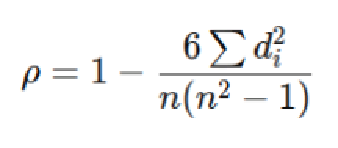
\includegraphics[scale=0.8]{figuras/CoeficientedeSpearman.pdf}
\end{center}


Em que:
\begin{itemize}
  \item \textbf{di:} Diferença entre os postos de cada par de observações,
  \item \textbf{n:} Número de observações.
\end{itemize}

Os valores do coeficiente de Spearman variam entre -1 e +1, com: 
\begin{itemize}
  \item \textbf{+1} indica uma correlação \textbf{monotônica positiva perfeita}: À medida que uma variável aumenta, a outra também aumenta de forma consistente.
  \item \textbf{-1} indica uma correlação \textbf{monotônica negativa perfeita}: À medida que uma variável aumenta, a outra diminui de forma consistente.
  \item \textbf{0} indica \textbf{nenhuma correlação monotônica}: Não há uma relação clara entre as duas variáveis, seja positiva ou negativa.
\end{itemize}

Utilizaremos esses valores para interpretar a força e a direção da relação entre as variáveis segundo \citeonline{santos2007} na tabela \ref{tab:correlacao_pearson}:

\begin{table}[h!]
  \centering
  \captionsetup{font=footnotesize, justification=centering, labelsep=period, position=above}
  \caption{ Interpretação do coeficiente de correlação de Spearman}
  \label{tab:correlacao_pearson}
  \begin{tabular}{|c|c|}
  \hline
  \vspace{0.2cm} \cellcolor[HTML]{C0C0C0} \textbf{Coeficiente de Correlação} & \cellcolor[HTML]{C0C0C0} \textbf{Correlação} \\
  \hline
  $R_{xy} = 1$ & Perfeita positiva \\
  \hline
  $0,8 \leq R_{xy} < 1$ & Forte positiva \\
  \hline
  $0,5 \leq R_{xy} < 0,8$ & Moderada positiva \\
  \hline
  $0,1 \leq R_{xy} < 0,5$ & Fraca positiva \\
  \hline
  $0 \leq R_{xy} < 0,1$ & Infima positiva \\
  \hline
  $0$ & Nula \\
  \hline
  $-0,1 \leq R_{xy} < 0$ & Infima negativa \\
  \hline
  $-0,5 \leq R_{xy} < -0,1$ & Fraca negativa \\
  \hline
  $-0,8 \leq R_{xy} < -0,5$ & Moderada negativa \\
  \hline
  $-1 \leq R_{xy} < -0,8$ & Forte negativa \\
  \hline
  $R_{xy} = -1$ & Perfeita negativa \\
  \hline
  \end{tabular}
  \caption*{\scriptsize Fonte: \cite{santos2007}}
\end{table}

Na base de dados, o coeficiente de Spearman será aplicado ao transformar os valores originais das variáveis em ranks e calcular a correlação entre eles usando a função \textit{spearmanr()} da biblioteca \textit{SciPy}. Isso permitirá identificar relações monotônicas entre as variáveis de forma robusta contra outliers. Com os resultados obtidos, determinaremos quais variáveis têm maior influência na previsão de euploidia e justificaremos com base nos coeficientes e nas visualizações geradas.

\end{apendicesenv}
